\documentclass[]{article}
\usepackage[a4paper]{geometry}
\renewcommand{\contentsname}{Table Of Contents}
\usepackage{amssymb}
\usepackage{hyperref}
\usepackage{fancyhdr}
\usepackage{graphicx}
\graphicspath{{./images/}}
\pagestyle{fancy}
\fancyhead{}
\fancyfoot{}
\fancyhead[L]{\slshape\MakeUppercase{Door Alarm System on Raspberry Pi 4}}
\fancyhead[R]{\slshape Angelo Barbera}
\fancyfoot[C]{\thepage}
\title{\huge Door Alarm System on Raspberry Pi 4}
\author{Angelo Barbera}
\date{February 20, 2023}

\begin{document}

\begin{titlepage}
	\centering
	{\scshape\LARGE Univeristà degli Studi di Palermo \par}
	\vspace{0.6cm}
	{\scshape\Large Embedded Systems \par}
	\vspace{1.8cm}
	{\huge\bfseries Door Alarm System on Raspberry Pi 4 \par}
	\vspace{2cm}
	\vfill
	{\large Angelo Barbera\par}
    \vspace{0.2cm}
    {\large February 20, 2023\par}
\end{titlepage}

\pagenumbering{roman}

\tableofcontents

\clearpage
\pagenumbering{arabic}


\section{Introduction}
The project is a Door Alarm System. The System is able to monitor the open or closed status of a door using a hall sensor
to detect the presence of a magnet; if the latter is far from the sensor, it is emitted a sound alert with a buzzer. 
Using two LEDs and a LCD 1602 the status of the door is shown. In addition there is a button that can be used to 
turn off the alarm when the door is closed.
\\ 
In the following sections is described in detail the hardware and the software used to implement the project.

\section{Hardware}

\subsection{Raspberry PI 4}

\begin{center}
    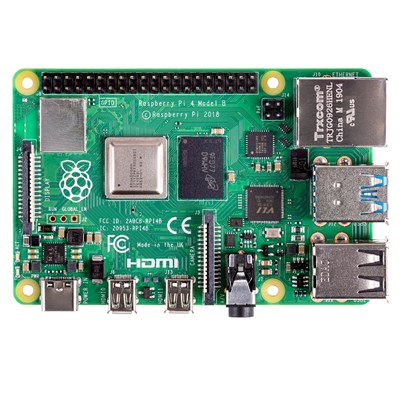
\includegraphics[scale=0.6]{raspberry_pi_4}
\end{center}
The chosen target for this project is the Raspberry Pi 4 Model B, a single board computer developed by 
the Raspberry Pi Foundation and realeased in 2019. The tech specs include:
\begin{itemize} 
    \item Broadcom BCM2711, Quad core Cortex-A72 (ARM v8) 64-bit SoC @ 1.5Ghz
    \item 1GB, 2GB, 4GB, or 8GB LPDDR4-3200 SDRAM (depending on model)
    \item 2.4 GHz and 5.0 Ghz 802.11ac wireless
    \item Gigabit Ethernet
    \item Bluetooth 5.0, BLE
    \item 2 USB 3.0 ports, 2 USB 2.0 ports
    \item Raspberry Pi standard 40 pin GPIO header
    \item 2 micro-HDMI ports (up to 4kp60 supported)
    \item 2-lane MIPI DSI display port
    \item 2-lane MIPI CSI camera port
    \item 4-pole stereo audio and composite video port
    \item H.265 (4kp60 decode), H.264 (1080p60 decode, 1080p30 encode)
    \item OpenGL ES 3.1, Vulkan 1.0
    \item Micro-SD card slot for loading operating system and data storage
    \item 5V DC via USB-C connector (minimum 3A)
    \item 5V DC via GPIO header (minimum 3A)
    \item Power over Ethernet (PoE) enabled (requires separate PoE HAT)
    \item Operating temperature 0 - 50 °C ambient
\end{itemize}

\subsection{FT232-AZ USB to TTL serial UART adapter}

\begin{center}
    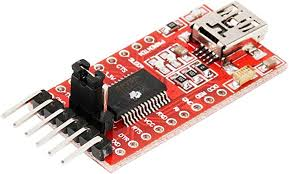
\includegraphics[scale=0.4]{uart_adapter}
\end{center}
The FT232-AZ USB to TTL serial UART adapter is used to connect the PC used during the development of the project
to the target in order to send and receive data between the PC and the Raspberry Pi 4. 
The PC is connected through a USB port, the target is connected through GPIO pins according to the 
following table.

\begin{center}
    \begin{tabular}{ |c|c|c| } 
        \hline
        GPIO & Function & UART adapter  \\
        \hline
        14 (Tx) & Output & Rx \\ 
        15 (Rx) & Input & Tx \\ 
        Ground & Ground & Ground \\ 
        \hline
    \end{tabular}
\end{center}

\subsection{KY-003 Hall sensor}

\begin{center}
    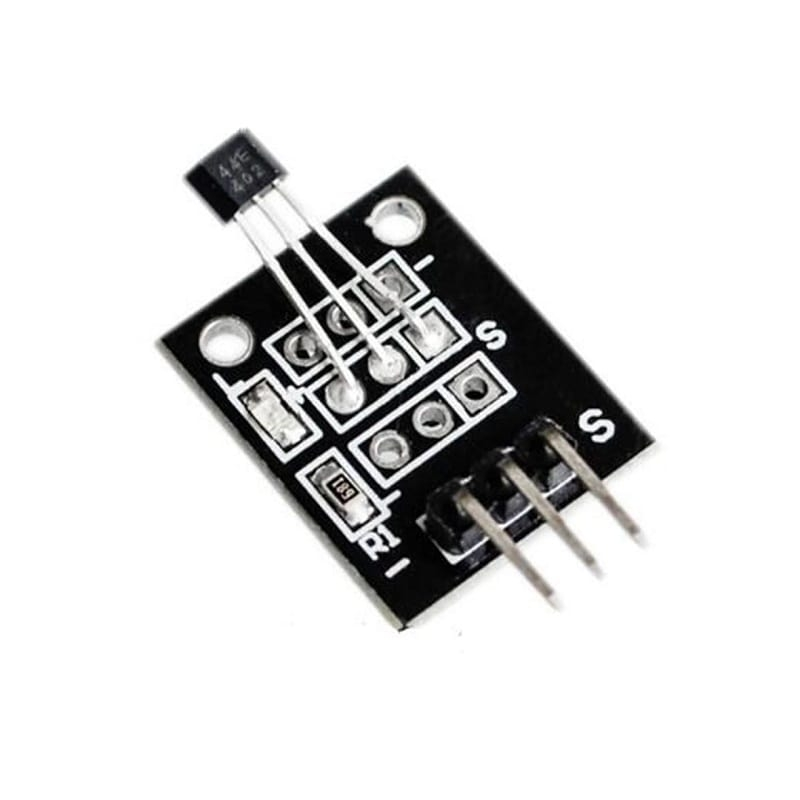
\includegraphics[scale=0.2]{ky-003}
\end{center}
The KY-003 hall sensor allows to detect a magnetic field. When the magnetic field at the Hall sensor exceeds
the operate point threshold (BOP) the output of the device switches low. When the magnetic field is reduced
to below the realease point threshold (BRP) the device output switches high.
BOP and BRP may vary respectively from 1 mT to 33 mT and from 5 mT to 35 mT at operating 
temperature T = 25° C depending on the sensor model.
This sensor is used to trigger the alarm when the magnet is far from the sensor.

\subsection{KY-012 Buzzer}

\begin{center}
    
\includegraphics[scale=0.4]{ky-012}
\end{center}
The KY-012 Buzzer is an active piezoelectric buzzer, it generates a sound of approximately 2.5kHz when 
input signal (S) is high. The Buzzer is activated when the Hall sensor does not detect the magnet.

\subsection{LEDs}

\begin{center}
    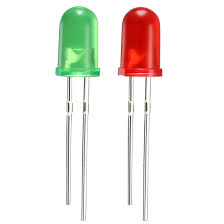
\includegraphics[scale=0.4]{leds}
\end{center}
The LEDs are used to show the alarm status. When the Hall sensor does not detects the magnet the green LED turns off 
and the red LED turns on. When the Hall sensor detect the magnet and the push button is pressed, the green LED turns on
and the red LED turns off.

\subsection{Push Button}

\begin{center}
    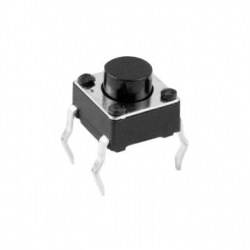
\includegraphics[scale=0.5]{push_button}
\end{center}
The push button can be used to turn off the alarm when the hall sensor detects the magnet.

\subsection{Resistors}

\begin{center}
    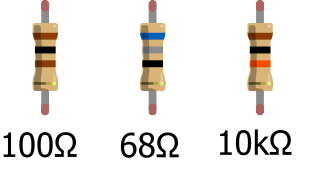
\includegraphics{resistors}
\end{center}
The 100 $ \Omega $ and 68 $ \Omega $ resistors are connected in series to the LEDs to limit the current flowing through the LED and to ensure that the supplied 
voltage does not exceeds the maximum voltage of the LED. The 100 $ \Omega $ resistor is connected to the red LED, the 68 $ \Omega $ 
resistor is connected to the green LED.
The 10k $ \Omega $ resistor is a pull-down resistor, it is used to prevent an undefined state for GPIO 25 when the button is not pressed.

\subsection{LCD 1602}

\begin{center}
    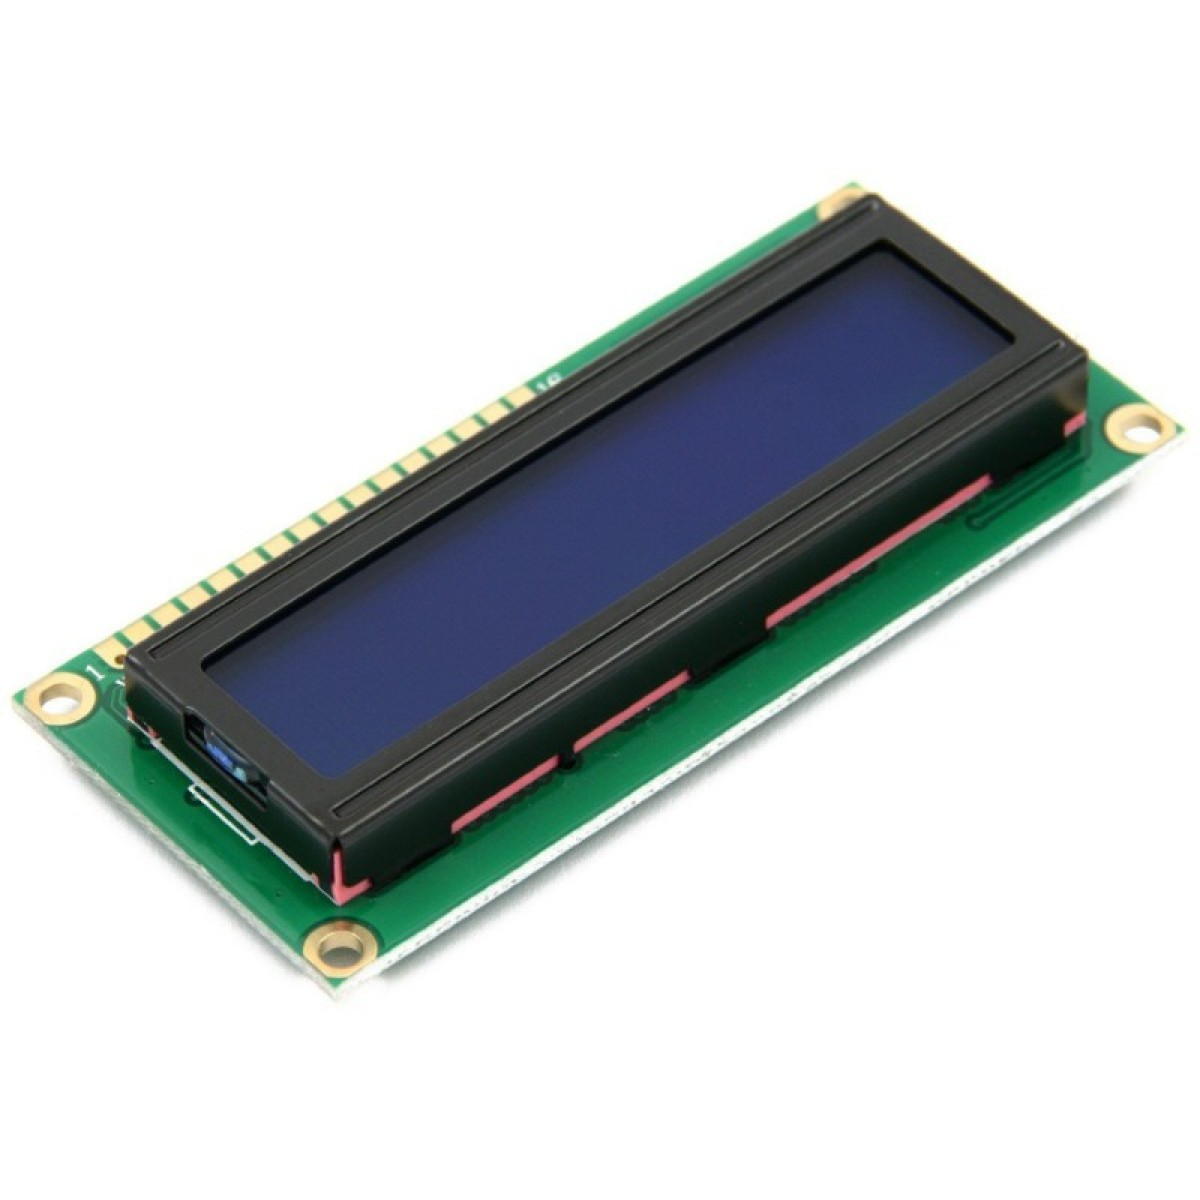
\includegraphics[scale=0.2]{lcd}
\end{center}
The LCD 1602 is an industrial character LCD that can display 16x02 or 32 characters at the same time. 
The LCD 1602 is controlled through a parrallel interface with 8-bit / 4-bit data bus and 3 control signals. 
The interface signals reach the two controller chips that drive the LCD panel as shown in the following block diagram.

\begin{center}
    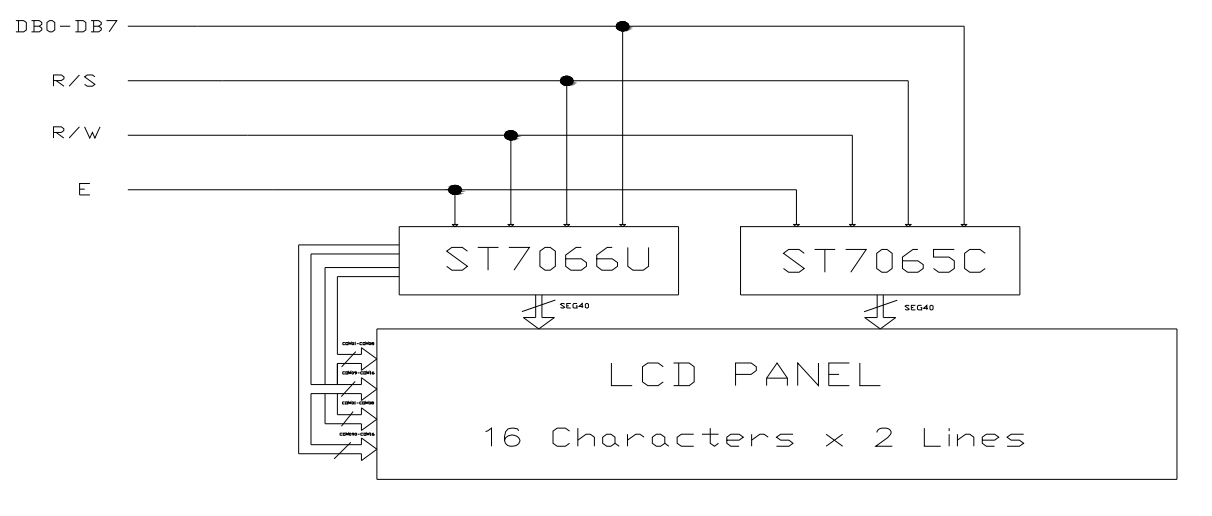
\includegraphics[scale=0.4]{lcd_block_diagram}
\end{center}
The following table describes the pin assignment

\begin{center}
    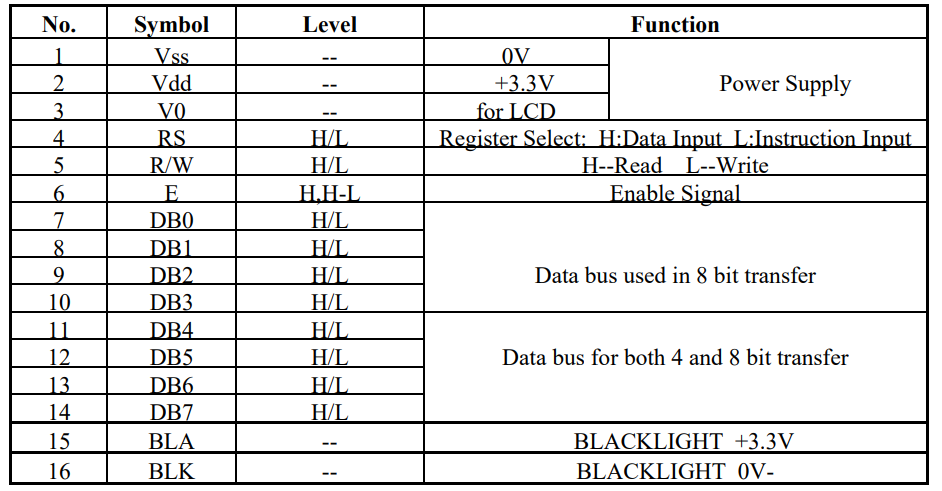
\includegraphics[scale=0.4]{lcd_pin_assignment}
\end{center}
The LCD module is controlled through instructions to set display format, data length, scrolling modality, internal RAM address, 
to perform data transfer from/to internal RAM and to access status flag. The following table describes the instructions.

\begin{center}
    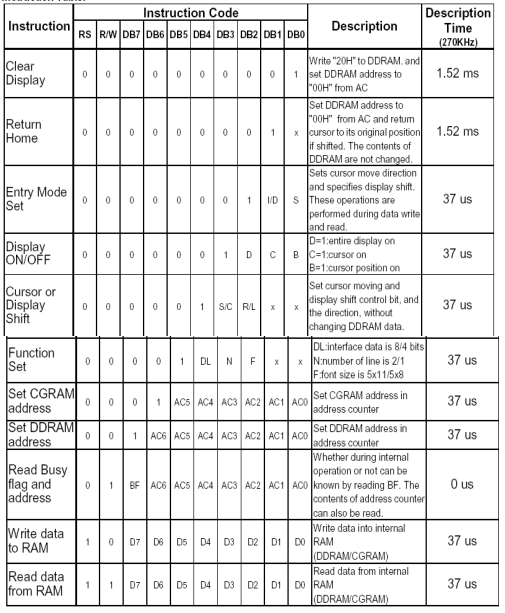
\includegraphics[scale=0.6]{lcd_instruction}
\end{center}
In order to write to the controller chips we need to set properly the control bits: the R/W bit must be set to 0 for writing,
the RS bit must be set to 1 for data input and to 0 for instruction input, the E bit must be set to 1 before the start of the data transmission
and must be set to 0 before the end of the data transmission as shown in the following figure

\begin{center}
    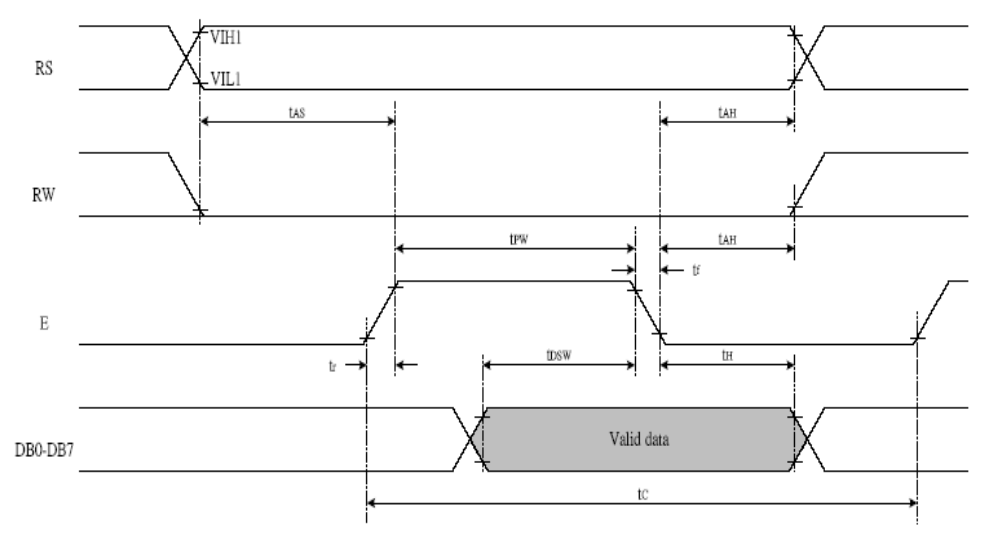
\includegraphics[scale=0.5]{lcd_writing}
\end{center}


\subsection{PCF8574AT 8-bit I/O expander for I2C bus}
\begin{center}
    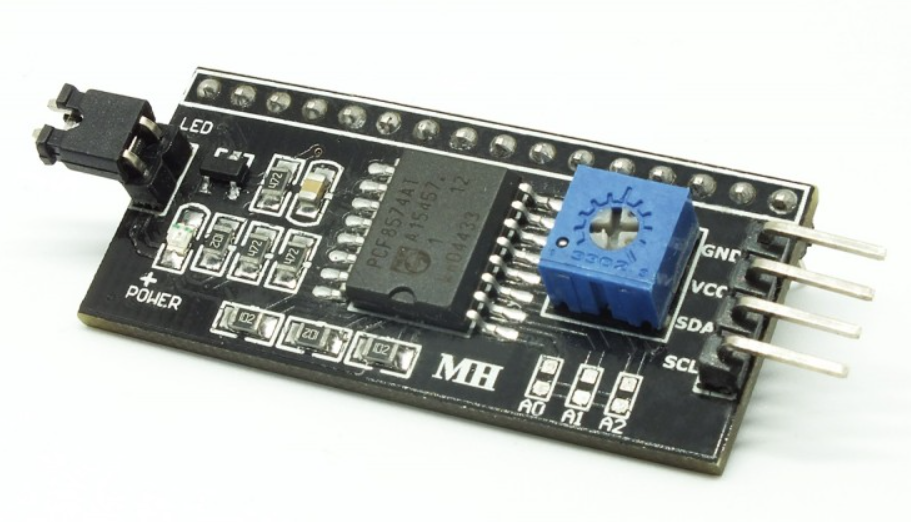
\includegraphics[scale=0.2]{io_expander}
\end{center}
The PCF8574AT provides general-purpose remote I/O expansion via the two-wire bidirectional $ I^2C $ bus. It is used to connect the Raspberry Pi to the LCD 1602
using the $ I^2 C $ bus instead of the parrallel interface.

\subsubsection{The I2C bus}
The $ I^2C $ bus is a synchronous, multi-master, multi-slave, packet switched, single-ended, serial computer bus invented by Philips Semiconductor.
It is used to connect lower speed peripheral integrated circuits to processors and microcontrollers in short distance. 
Each device connected to the bus is software addressable by a unique address to differentiate between other devices that are on the same bus. 
Two wires carry data (SDA) and clock signal (SCL). \\
Open drain connection allows for bidirectional communication: to transmit low the logic activate the pull-down FET (so the line is pulled low), 
to transmit high the logic realease the bus turning off the pull-down FET (so the pull-up resistor pulls up the line). \\
The procedure for a master to send data to a slave is the following: 
\begin{itemize}
    \item Master-transmitter sends a START condition and addresses the slave-receiver 
    \item Master-transmitter sends data to slave-receiver 
    \item Master-transmitter terminates the transfer with a STOP condition 
\end{itemize}
The START condition is defined by a high-to-low transition on the SDA line while the SCL is high. The STOP condition is defined by a low-to-high transition 
on the SDA line while the SCL is high.

\begin{center}
    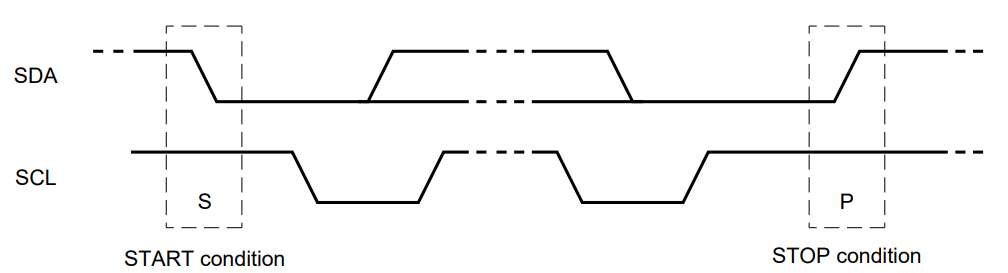
\includegraphics[scale=0.5]{start_stop_conditions}
\end{center}
One data bit is transferred during each clock pulse of the SCL, the data on the SDA line must remain stable duriong the high period of the clock pulse
as changes in the data line at this time will be interpreted as control signals (START or STOP). Data is transferred Most Significant Bit first. 
Any number of data bytes can be transferred between the START and STOP conditions.

\begin{center}
    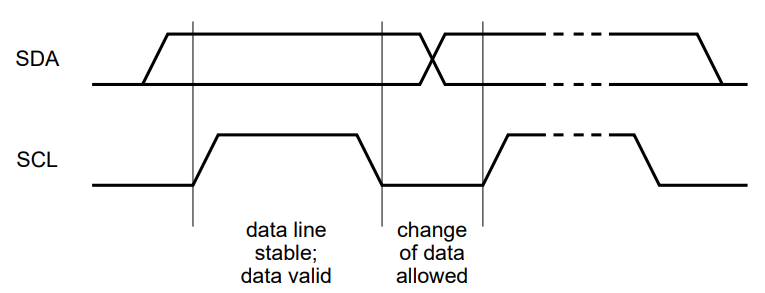
\includegraphics[scale=0.5]{bit_transfer}
\end{center}
Each byte of data is followed by one ACK (acknowledge) bit from the receiver to signal that the byte was successfully received. Before the receiver can send an ACK 
the transmitter must realease the SDA line. To send an ACK bit the receiver pulls down the SDA after receiving the last bit so the line is stable low during the high 
fase of the ACK clock period. When SDA line remains high after receiving the last bit, this is interpreted as a NACK (not acknowledge)

\begin{center}
    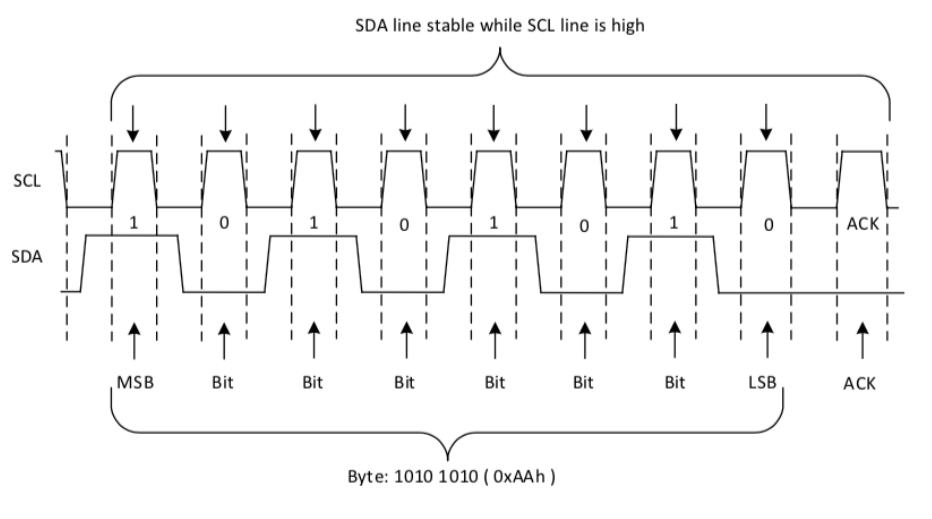
\includegraphics[scale=0.5]{byte_transmission}
\end{center}

The procedure to write on the bus is the following:
\begin{itemize}
    \item The master sends a START condition with the slave's address followed by the R/W bit set to 0
    \item The slave sends the acknowledge bit 
    \item The master sends the register address of the register it whishes to write to 
    \item The slave acknowledges the register address
    \item The master starts sending the register data to the slave 
    \item The master terminates the transmission with a STOP condition
\end{itemize}

\begin{center}
    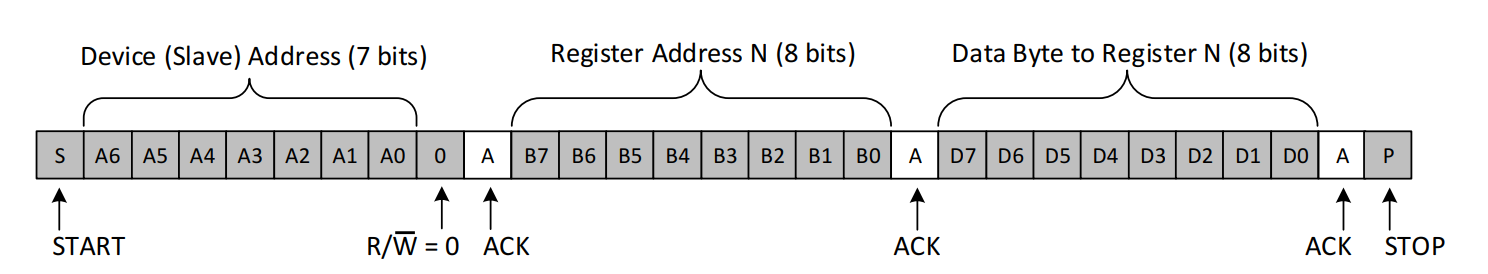
\includegraphics[scale=0.4]{write_procedure}
\end{center}

\subsubsection{LCD connection}
The following table describes the connections between the LCD 1602 and the PCF8574AT 

\begin{center}
    \begin{tabular}{|c|c|} 
        \hline
        PCF8574AT & LCD 1602 \\
        \hline
        P0 & RS \\
        P1 & RW \\
        P2 & E \\
        P3 & Backlight \\
        P4 & D4 \\
        P5 & D5 \\
        P6 & D6 \\
        P7 & D7 \\
        \hline
    \end{tabular}
\end{center}

In order to set the LCD 1602 to 4 bit mode it is necessary to send the following command 

\begin{center}
    \begin{tabular}{|c|c|c|c|c|c|c|c|c|} 
        \hline
        & D7 & D6 & D5 & D4 & Backlight & E & R/W & RS \\
        \hline
        2C & 0 & 0 & 1 & 0 & 1 & 1 & 0 & 0 \\
        28 & 0 & 0 & 1 & 0 & 1 & 0 & 0 & 0 \\
        \hline
    \end{tabular}
\end{center}

Now is possible to send a command signal or a data signal according to the following tables

\begin{center}
    \begin{tabular}{|c|c|c|c|c|c|c|c|c|} 
        \hline
        & D7 & D6 & D5 & D4 & Backlight & E & R/W & RS \\
        \hline
        MSB\_CMD C & B7 & B6 & B5 & B4 & 1 & 1 & 0 & 0 \\
        MSB\_CMD 8 & B7 & B6 & B5 & B4 & 1 & 0 & 0 & 0 \\
        LSB\_CMD C & B3 & B2 & B1 & B0 & 1 & 1 & 0 & 0 \\
        LSB\_CMD 8 & B3 & B2 & B1 & B0 & 1 & 0 & 0 & 0 \\
        \hline
    \end{tabular}
\end{center}

\begin{center}
    \begin{tabular}{|c|c|c|c|c|c|c|c|c|} 
        \hline
        & D7 & D6 & D5 & D4 & Backlight & E & R/W & RS \\
        \hline
        MSB\_DATA D & B7 & B6 & B5 & B4 & 1 & 1 & 0 & 1 \\
        MSB\_DATA 9 & B7 & B6 & B5 & B4 & 1 & 0 & 0 & 1 \\
        LSB\_DATA D & B3 & B2 & B1 & B0 & 1 & 1 & 0 & 1 \\
        LSB\_DATA 9 & B3 & B2 & B1 & B0 & 1 & 0 & 0 & 1 \\
        \hline
    \end{tabular}
\end{center}


\subsection{GPIO wiring diagram}

\begin{center}
    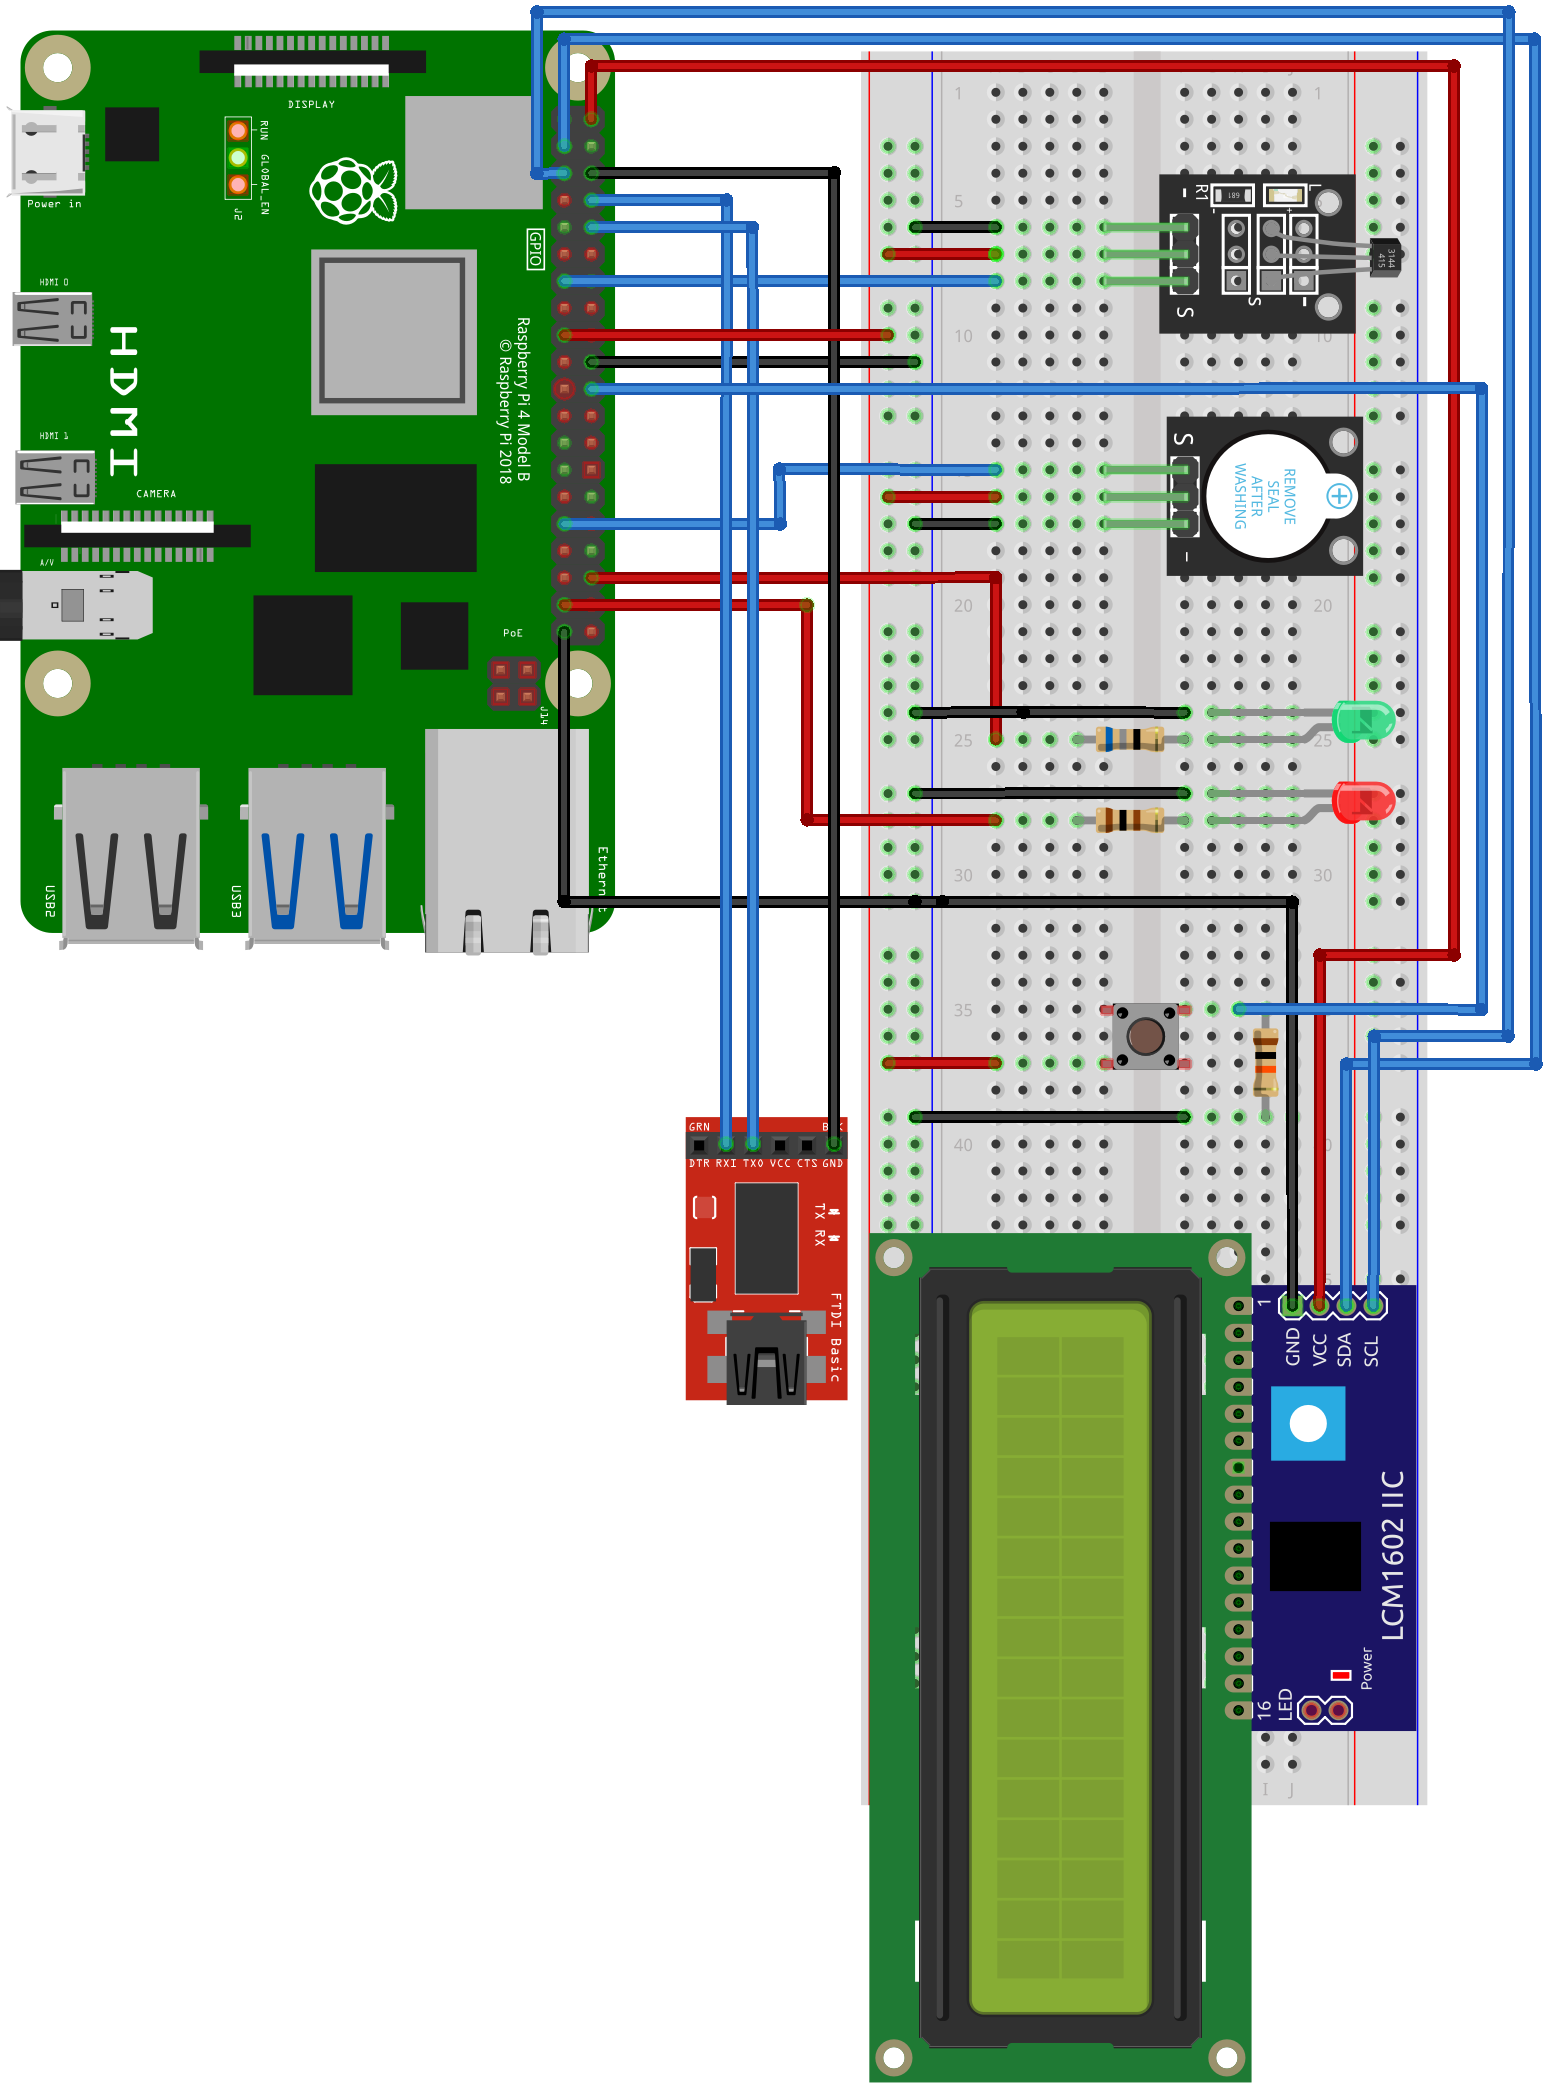
\includegraphics[scale=0.9]{breadboard}
\end{center}

\newpage
The following table is the GPIO wiring diagram.

\begin{center}
    \begin{tabular}{ |c|c|c| } 
        \hline
        GPIO & Function & Connection \\
        \hline
        2 & SDA & SDA (I/O expander) \\
        3 & SCL & SCL (I/O expander) \\
        6 & Output & S (Buzzer) \\
        16 & Output & Anode (Green LED) \\
        25 & Input & Button \\
        26 & Output & Anode (Red LED) \\
        27 & Input & S (Hall sensor) \\
        5V & Power & VCC (I/O expander) \\
        3V3 & Power & Breadboard \\
        Ground & Ground & Breadboard \\
        \hline
    \end{tabular}
\end{center}

\section{Environment}

\subsection{pijForthos}
Forth is a procedural, stack-oriented programming lenguage and interactive environment designed by Charles H. "Chuck" Moore. Forth combines
a compiler with an integrated command shell, where the user interacts via subroutine called words. \\
PijForthos is a bare-metal operating system for Raspberry Pi based on Jonesforth-ARM. Jonesforth-ARM is an ARM port of x86 JonesForth 
by Richard W.M. Jones, a Forth interpreter developed for ARM. If you have pijFORTHos on a Micro SD card in the Raspberry Pi, you can connect
it to development machine using the USB to TTL serial UART adapter. Using the programs described below you can have access to 
the Forth console.


\subsection{Minicom, Picocom}
Minicom is a text-based terminal emulator program for Unix-lile operating systems, it is used to set up a remote serial console.
Picocom is similar to Minicom and it was designed to serve as a simple, manual, modem configuration, testing and debugging tool. \\
ASCII-XFR transfers files in ASCII mode and it is used to send the source file to the Raspberry Pi allowing to set a delay between each character and line sent. It is useful
beacuse, since the UART connection is asynchronous, if the reciver is busy compiling or executing Forth words and the transmitter is sending data,
it is possible to lose them.  \\
The following command is used to set up the communication with the Raspberry Pi : \\
\texttt{picocom --b 115200 /dev/ttyUSB0 --imap delbs -s "ascii-xfr -sv -l100 -c10"}

\begin{itemize}
    \item \texttt{--b 115200} defines the baud rate
    \item \texttt{/dev/ttyUSB0} specifies the UART port
    \item \texttt{--imap delbs} maps del to backspace
    \item \texttt{-s "ascii-xfr -sv -l100 -c10"} specifies the external program that will be used to transmitting files
    \item \texttt{-sv} specifies verbose mode 
    \item \texttt{-l100} specifies the delay (100 milliseconds) after transmitting each line
    \item \texttt{-c10} specifies the delay (10 milliseconds) after transmitting each character
\end{itemize}

\section{Software}

\subsection{Environment setup}
To setup the environment it is necessary to format the micro SD card using FAT32 as file system. Then the following files must be copied in the micro SD card: 
\begin{itemize}
    \item \texttt{bootcode.bin} contains the bootloader code 
    \item \texttt{config.txt} contains the configuration parameters
    \item \texttt{start4.elf} contains the second-stage bootloader 
    \item \texttt{fixup.dat} contains Video Core code and initialization data 
    \item \texttt{bcm2711-rpi-4-b.dtb} describes the hadrware present in the Raspberry Pi
    \item \texttt{kernel7.img} contains the pijFORTHos code   
\end{itemize}
The \texttt{config.txt} file must be edited specifying the following settings:
\begin{itemize}
    \item \texttt{dtparam=i2c\_arm=on} enables $ I^2C $
    \item \texttt{enable\_uart=1} enables UART 
\end{itemize}

\subsection{Code structure}
The code is devided into the following files 

\begin{itemize}
    \item \texttt{se-ans.f} contains some definition for ANS compliance 
    \item \texttt{utils.f} contains utility words
    \item \texttt{i2c.f} contains the words used to set up i2c 
    \item \texttt{lcd.f} contains the words used to control the lcd
    \item \texttt{peripherals.f} contains the words used to manage the peripherals
    \item \texttt{main.f} contains the words used to run the system 
\end{itemize}
The provious files must be sent to the Raspberry Pi using picocom in the specified order.

\subsubsection{se-ans.f}
\begin{verbatim}
\ Sistemi Embedded 18/19
\ Daniele Peri - Universita' degli Studi di Palermo
\
\ Some definitions for ANS compliance
\
\ v. 20181215

: JF-HERE   HERE ;
: JF-CREATE   CREATE ;
: JF-FIND   FIND ;
: JF-WORD   WORD ;

: HERE   JF-HERE @ ;
: ALLOT   HERE + JF-HERE ! ;

: [']   ' LIT , ; IMMEDIATE
: '   JF-WORD JF-FIND >CFA ; 

: CELL+  4 + ;

: ALIGNED   3 + 3 INVERT AND ;
: ALIGN JF-HERE @ ALIGNED JF-HERE ! ;

: CREATE   JF-WORD JF-CREATE DOCREATE , ;
: (DODOES-INT)  ALIGN JF-HERE @ LATEST @ >CFA ! DODOES> ['] LIT ,  
  LATEST @ >DFA , ; 
: (DODOES-COMP)  (DODOES-INT) ['] LIT , , ['] FIP! , ; 
: DOES>COMP   ['] LIT , HERE 3 CELLS + , ['] (DODOES-COMP) , ['] EXIT , ;
: DOES>INT   (DODOES-INT) LATEST @ HIDDEN ] ;
: DOES>   STATE @ 0= IF DOES>INT ELSE DOES>COMP THEN ; IMMEDIATE
\end{verbatim}

\subsubsection{utils.f}

\begin{verbatim}
HEX

FE200000 CONSTANT PERI_BASE    \ Base address of peripherals
1 CONSTANT OUTPUT   
0 CONSTANT INPUT 

\ Creates a busy loop
: DELAY ( delay_value -- )
    BEGIN 1 - DUP 0 = UNTIL DROP 
;

\ Returns the GPFSEL address of the specified fsel number
: FSEL>ADDRESS ( fsel_number -- gpfsel_register_address ) 
    A / 4 * PERI_BASE + 
;

\ Returns the GPFSEL value of the specified fsel number
: FSEL>VALUE ( fsel_number -- gpfsel_register_value )
    FSEL>ADDRESS @
;

\ Creates bit mask to safely modify GPIO registers value
: MASK ( fsel_number value -- bit_mask)  
    SWAP A MOD 3 * LSHIFT
; 

\ Returns the new_value setting to 0 the specified bit in mask
: BIC ( value mask - new_value)
    INVERT AND
;

\ Creates bit mask to use bic (bit clear)
: BIC_MASK ( fsel_number -- bic_mask )
    7 MASK 
;

\ Gets only the first 4 MSB from a byte
: MSB ( byte -- MSB)
    4 RSHIFT 
;

\ Gets only the first 4 LSB from a byte
: LSB ( byte -- LSB)
    0F AND 
;

\ Copies the top of the return stack wihout affecting it
: R@ ( -- TORS )
    R> R> TUCK >R >R
;
 
\ Sets GPFSEL register to the specified value
: SET_GPFSEL ( fsel_number value -- )   
    OVER                         \ ( fsel_number value fsel_number ) 
    BIC_MASK                     \ ( fsel_number value bic_mask ) 
    ROT ROT SWAP DUP ROT         \ ( bic_mask fsel_number fsel_number value )
    MASK                         \ ( bic_mask fsel_number bit_mask ) 
    SWAP                         \ ( bic_mask bit_mask fsel_number ) 
    DUP                          \ ( bic_mask bit_mask fsel_number fsel_number )
    FSEL>VALUE                   \ ( bic_mask bit_mask fsel_number original_value )
    >R ROT R> SWAP               \ ( bit_mask fsel_number original_value bic_mask )
    BIC                          \ ( bit_mask fsel_number bic_value ) 
    ROT                          \ ( fsel_number bic_value bit_mask )
    OR                           \ ( fsel_number new_value )
    SWAP                         \ ( new_value fsel_number )
    FSEL>ADDRESS                 \ ( new_value fsel_address )
    !      
;

\ Returns the mask used to set or clear GPIO register
: SET_CLR_MASK ( gpio_pin -- mask )
    DUP 20 < IF 1 SWAP LSHIFT                     \ gpio_pin < 32
    ELSE DUP 1F > IF 1 SWAP 20 MOD LSHIFT         \ gpio_pin > 31
    THEN THEN 
;

\ Sets GPIO register 
: ON ( gpio_pin -- )
    DUP SET_CLR_MASK SWAP
    DUP 20 < IF DROP 1C PERI_BASE + !             \ gpio_pin < 32
    ELSE DUP 1F > IF DROP 20 PERI_BASE + !        \ gpio_pin > 31
    THEN THEN 
;

\ Clears GPIO register 
: OFF ( gpio_pin -- )
    DUP SET_CLR_MASK SWAP
    DUP 20 < IF DROP 28 PERI_BASE + !             \ gpio_pin < 32
    ELSE DUP 1F > IF DROP 2C PERI_BASE + !        \ gpio_pin > 31
    THEN THEN 
;

\ Returns the value of the specified pin
: READ ( gpio_pin -- value )
    DUP 20 < IF 34 PERI_BASE + @ SWAP RSHIFT 1 AND 
    ELSE DUP 1F > IF 38 PERI_BASE + @ SWAP RSHIFT 1 AND 
    THEN THEN 
;
\end{verbatim}

\subsubsection{i2c.f}

\begin{verbatim}
HEX

FE804000 CONSTANT BSC1                   \ Base address of BSC1 register
BSC1 CONSTANT CONTROL                   \ Control register address
4 BSC1 + CONSTANT STATUS                \ Status register address
8 BSC1 + CONSTANT DATA_LENGTH           \ Data Length register address
0C BSC1 + CONSTANT SLAVE_ADDRESS        \ Slave Address register address
10 BSC1 + CONSTANT DATA_FIFO            \ Data FIFO register address

\ Sets GPIO2 and GPIO3 to ALT0
: CONFIG_I2C_GPIO ( -- )
    2 4 SET_GPFSEL          \ Sets FSEL2 to 100
    3 4 SET_GPFSEL          \ Sets FSEL3 to 100 
;

\ Resets the Status Register setting:
\ bit 1 (Transfer Done) to 1,
\ bit 8 (Ack Error) to 1,
\ bit 9 (Clock Stretch Timeout) to 1
: RESET_STATUS ( -- )
    STATUS @ 302 OR STATUS !
;

\ Resets FIFO setting bit 4 (FIFO Clear) to 1
: RESET_FIFO ( -- )
    CONTROL @ 10 OR CONTROL !
;

\ Sets the number of bytes of data to transmit or receive to 1
: SET_DATA_LENGTH ( -- )
    DATA_LENGTH @ 1 OR DATA_LENGTH !
;

\ Sets the slave address 
: SET_SLAVE ( -- )
    SLAVE_ADDRESS @ 7F BIC 27 OR SLAVE_ADDRESS !
;

\ Stores data in Data FIFO register
: STORE_FIFO ( data -- )
    DATA_FIFO @ FF BIC OR DATA_FIFO !
;

\ Starts a new transfer setting 
\ bit 0 (Read Transfer) to 0
\ bit 7 (Start Transfer) to 1 
\ bit 15 (I2C enable) to 1 
: START_TRANSFER ( -- )
    CONTROL @ 1 BIC 8080 OR CONTROL !
;

\ Sends 8 bit using i2c
: SEND ( data -- )
    RESET_STATUS 
    RESET_FIFO
    SET_DATA_LENGTH
    SET_SLAVE
    STORE_FIFO
    START_TRANSFER
;

\end{verbatim}

\subsubsection{lcd.f}

\begin{verbatim}
HEX

02 CONSTANT FUNCTION_SET        \ Sets 4 bit mode
01 CONSTANT CLEAR               \ Clear lcd 

: DOOR ( -- reversed_ascii_code length)
    20 52 4F 4F 44 5 
;

: CLOSED ( -- reversed_ascii_code length)
    20 44 45 53 4F 4C 43 7
;

: OPEN ( -- reversed_ascii_code length)
    20 4E 45 50 4F 5
;

\ Sends a nibble to lcd 
: SEND_NIBBLE ( LSB settings -- )
    SWAP 4 LSHIFT OR
    SEND
    1000 DELAY
;

\ Sends command to lcd 
\ It is necessary to send: D7, D6, D5, D4, 
\ Backlight, Enable, Read (1)/Write (0), Register Select (1-data 0-instruction)
\ C = 1100, 8 = 1000
\ 4 MSB|C 
\ 4 MSB|8
\ 4 LSB|C
\ 4 LBS|8
: SEND_COMMAND ( command -- )
    DUP MSB SWAP LSB SWAP DUP              \ ( LSB MSB MSB )
    0C SEND_NIBBLE 
    08 SEND_NIBBLE 
    DUP 
    0C SEND_NIBBLE
    08 SEND_NIBBLE
;

\ Sends data to lcd 
\ It is necessary to send: D7, D6, D5, D4, 
\ Backlight, Enable, Read (1)/Write (0), Register Select (1-data 0-instruction)
\ D = 1101, 9 = 1001
\ 4 MSB|D
\ 4 MSB|9
\ 4 LSB|D
\ 4 LBS|9
: SEND_DATA ( data -- ) 
    DUP MSB SWAP LSB SWAP DUP              \ ( LSB MSB MSB )
    0D SEND_NIBBLE  
    09 SEND_NIBBLE 
    DUP 
    0D SEND_NIBBLE
    09 SEND_NIBBLE 
;

\ Initializes lcd 
: INITIALIZE_LCD ( -- )
    CONFIG_I2C_GPIO
    FUNCTION_SET SEND_COMMAND
;

\ Send a word to lcd
: SEND_WORD ( reversed_ascii_code length --)
    >R 
    BEGIN R> 1 - >R SEND_DATA R@ 0 = UNTIL 
    R> DROP
;

\end{verbatim}

\subsubsection{peripherals.f}

\begin{verbatim}
HEX

1A CONSTANT RED_LED                 \ The red LED is connected to GPIO 26
10 CONSTANT GREEN_LED               \ The green LED is connected to GPIO 16
6 CONSTANT BUZZER                   \ The Buzzer is connected to GPIO 6
19 CONSTANT BUTTON                  \ The Button is connected to GPIO 25
1B CONSTANT HALL_SENSOR             \ The Hall sensor is connected to GPIO 27


\ Initializes peripherals 
: INITIALIZE_PERIPHERALS ( -- )
    RED_LED OUTPUT SET_GPFSEL       \ Sets gpfsel 26 to output 
    GREEN_LED OUTPUT SET_GPFSEL     \ Sets gpfsel 16 to output 
    BUZZER OUTPUT SET_GPFSEL        \ Sets gpfsel 6 to output 
    BUTTON INPUT SET_GPFSEL         \ Sets gpfsel 25 to input 
    HALL_SENSOR INPUT SET_GPFSEL    \ Sets gpfsel 27 to input 
;

\ Returns the status of the button (1 or 0)
: BUTTON_STATUS ( -- button_status)
    BUTTON READ 
;

\ Returns the status of the hall sensor (1 or 0)
: HALL_SENSOR_STATUS  ( -- hall_sensor_status)
    HALL_SENSOR READ
;

\ Returns the status of the buzzer (1 or 0)
: BUZZER_STATUS ( -- buzzer_status )
    BUZZER READ
;
\end{verbatim}

\subsubsection{main.f}

\begin{verbatim}
HEX

\ Executes the program
HEX

\ Executes the program
: RUN ( -- )
    INITIALIZE_LCD
    CLEAR SEND_COMMAND          \ Sends clear command to LCD
    INITIALIZE_PERIPHERALS      
    GREEN_LED ON                \ Turns on the green LED
    
    BEGIN  \If the hall sensor does not detect the magnet and the alarm is off
        HALL_SENSOR_STATUS 1 = BUZZER_STATUS 0 = AND IF   
            GREEN_LED OFF       
            RED_LED ON 
            BUZZER ON
            CLEAR SEND_COMMAND
            DOOR OPEN SEND_WORD SEND_WORD    \ Sends words to LCD
        THEN \If the hall sensor detects the magnet, the alarm is on, the button is pressed  
        BUTTON_STATUS 1 = HALL_SENSOR_STATUS 0 = BUZZER_STATUS 1 = AND AND IF
            RED_LED OFF             
            GREEN_LED ON 
            BUZZER OFF
            CLEAR SEND_COMMAND
            DOOR CLOSED SEND_WORD SEND_WORD    \ Sends words to LCD
        THEN
    AGAIN
;

\end{verbatim}

\newpage

\section{References}

\begin{itemize}
    \item raspberrypi.com/products/raspberry-pi-4-model-b/specifications
    \item cdn.shopify.com/s/files/1/1509/1638/files/FT232-AZ\_Adapter\_Datenblatt\_AZ-Delivery-
    \\\_Vertriebs\_GmbH.pdf
    \item cdn.shopify.com/s/files/1/1509/1638/files/Hall\_Sensor\_Modul\_Digital\_Datenblatt.pdf
    \item cdn.shopify.com/s/files/1/1509/1638/files/KY-012\_Buzzer\_Modul\_Aktiv\_Datenblatt-
    \\\_AZ-Delivery\_Vertriebs\_GmbH.pdf
    \item wiki.52pi.com/index.php?title=Z-0234
    \item msb-co.ir/wp-content/uploads/2021/10/eone-1602a1.pdf
    \item nxp.com/docs/en/data-sheet/PCF8574\_PCF8574A.pdf
    \item ti.com/lit/an/slva704/slva704.pdf
    \item github.com/organix/pijFORTHos
    \item linux.die.net/man/1/minicom
    \item linux.die.net/man/8/picocom
    \item linux.die.net/man/1/ascii-xfr
    \item manpages.ubuntu.com/manpages/trusty/man8/picocom.8.html
    \item unix.com/man-page/redhat/1/ascii-xfr/
\end{itemize}



\end{document}